
\chapter{実験と考察}

この章では,これまでに述べたwildcardを許容することで頻出部分グラフマイニング
による出力がどれほど増え,出力時間が長くなるかを実験する.
さらに,提案した飽和・極大パターンにより,どれほど出力が抑えられるか,
出力時間はどのように変化するかを実験,検証する.

また,wildcardを許容した部分グラフパターンがどれほど有用であるかを,
機械学習の特徴として用いることで検証する.

\section{実験環境}
本手法を実装したものの実験環境として,以下を使用した.

\begin{center}
\begin{tabular}{cl}
\hline
CPU& Intel(R) Core(TM) i7-3770K 3.50GHz\\
\hline
メモリ&33GB\\
\hline
OS &Ubuntu 14.04.3 LTS\\
\hline
\end{tabular}
\end{center}

\section{使用したデータベース}
今回,Takigawaら\cite{deltol}によって用いられたMutagとCPDBの2つのデータを使用し,実験を行った.
それぞれのデータベースのグラフ数,平均ノード数,平均エッジ数を表\ref{dataset}に示す.AIDS(CAvsCM)
に関しては,機械学習に対する実験で使用した.
\begin{table}[h]
\caption{使用したデータセット}
\begin{center}
\begin{tabular}{|c|l|l|l|}
\hline
 &グラフ数&平均ノード数&平均エッジ数\\
\hline
Mutag &188&17.9&19.8\\
\hline
CPDB&684&14.1&14.6\\
\hline
AIDS(CAvsCM)&1503&59.0&61.6\\
\hline
\end{tabular}
\end{center}
\label{dataset}
\end{table}
\section{出力数と出力時間に関する実験}
\label{out-exp}

頻出部分グラフマイニングにwildcardを許容した場合の出力数,CPUtimeの比較を行う.
さらに増加した出力数が,wildcard許容版$\delta$-tolerance closed frequent subgraphs algorithmによって抑えられているのか実験した結果を出力数とCPUtimeの観点から検証する.

この実験では頂点のラベルにのみwildcardを許容した.これは使用するデータが化合物データであり,化合物データにおいて辺のラベルは
結合数を指すことが多いため,辺のラベルにwildcardを考える必要はないと判断したためである.
しかし,一般的なグラフデータベースにとって辺のラベルが重要な情報を持つことは少なくないため,
辺のラベルに対してwildcardを許容するべき時もあるが,これは頂点のラベルと同様に拡張可能である.


図\ref{cpdb}に実験結果を示す.
図\ref{cpdb}左がMutag,図\ref{cpdb}右がCPDBの実験結果で,それぞれ上図が出力数,
中央図がCPUtime,下図が1出力あたりのCPUtimeの実験結果を表している.
図中においてgSpanは通常の頻出部分グラフマイニング,
gSpan with wildcardはwildcardを1つ許容した頻出部分グラフマイニング,
closed with wildcard,maximal with wildcardはそれぞれ
wildcardを1つ許容した頻出部分グラフマイニングに対する
頻出飽和パターン集合,頻出極大パターン集合の結果である.

\subsection{考察}

Mutagの実験結果では,図\ref{cpdb}左において,gSpanとgSpan with wildcardを比較すると,
misupをさげるとどちらも指数的に出力が伸びているのに対し,
minsupを固定して比較すると,出力数はほぼ定数倍であることがわかる.
CPDBの結果でも同様のことが言え,
これはすべての頻出部分グラフのすべての頂点ラベルに対して
wildcardを許容した場合を考えることができるためであり,
通常の頻出部分グラフに対して出力部分グラフの平均ノード数倍の出力が得られるものと考えられる.
またCPUtimeにおいて,gSpanとgSpan with wildcardを比較すると,
図\ref{cpdb}の左右の中央図より,
こちらもほぼ定数倍で増えていることがわかる.
これは図\ref{cpdb}の下図より見て取れるように
,gSpanとgSpan with wildcardの1つあたりのCPUtimeはほぼ同じであるためである.

実験結果より,頻出部分グラフマイニングではminsupを下げると指数倍以上に出力が増える.
さらに,wildcardを許容することでほぼ定数倍ではあるが出力数が増え,扱いがより困難になると考えられる.
そこで飽和・極大パターン集合による集合要約の効果を検証する.

まずはMutagとCPDBのデータの違いによる差をみると,
MutagはCPDBに比べデータ数は少ないが平均のグラフサイズが大きく,
頻出部分グラフマイニングから見られるように出力数が多いことから
似たグラフが多いことがみてとれる.
それに比べCPDBではグラフデータベースが疎であるためか,
頻出部分グラフがMutagに比べて少ない.

図\ref{cpdb}の左右の上図,中央図より,
飽和・極大パターン集合を求めると通常の部分グラフパターンより時間がかかるが,
出力はかなり抑えられていることが,実験結果よりわかる.
さらに$\delta$の指標により飽和と極大の集合間の出力を
自由に決めることができる.今回の実験では,$\delta$を変えた実験は追加していない
が,原理上,飽和と極大の間になる.

図\ref{cpdb}の左右の下図より,
MutagとCPDBの両者に見られるようにwildcardを許容した頻出部分グラフの
飽和・極大パターン集合は頻出部分グラフの増加傾向ほど
増えないためminsupをさげると通常の頻出部分グラフ数ほどの出力まで抑えられている.
さらにMutagはCPDBに比べ似たグラフが多いためその傾向が顕著にあらわれている.
図\ref{cpdb}右の中央図からわかるように,
CPUtimeでは出力数が増えた場合,枝刈りが有効で,
wildcardを許容した頻出部分グラフマイニングに対して
飽和・極大パターン集合のほうが時間がかからなくなることもある.

\begin{figure}[H]
\begin{tabular}{cc}
      Mutag &  CPDB \\ 
    \begin{minipage}{80mm}
      \centering
      \scalebox{1.1}{\includegraphics{fig/mutag_out.eps}}
    \end{minipage} &
    \begin{minipage}{80mm}
      \centering
      \scalebox{1.1}{\includegraphics{fig/cpdb_out.eps}}
    \end{minipage} \\ 
    \begin{minipage}{80mm}
      \centering
      \scalebox{1.1}{\includegraphics{fig/mutag_time.eps}}
    \end{minipage} &
    \begin{minipage}{80mm}
      \centering
      \scalebox{1.1}{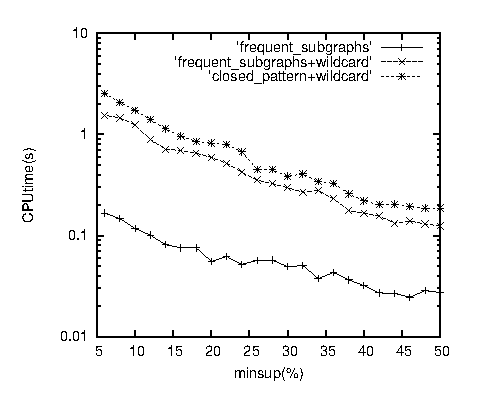
\includegraphics{fig/cpdb_time.eps}}
    \end{minipage} \\
    \begin{minipage}{80mm}
      \centering
      \scalebox{1.1}{\includegraphics{fig/per_mutag.eps}}
    \end{minipage} &
    \begin{minipage}{80mm}
      \centering
      \scalebox{1.1}{\includegraphics{fig/per_cpdb.eps}}
    \end{minipage} \\

  \end{tabular}
\caption{Mutag(左)CPDB(右)の実験結果:上から順に出力数,CPUtime,1出力あたりのCPUtime}
\label{cpdb}
\end{figure}

%\newpage
\section{機械学習に対する応用実験}
本節では,実験に用いたデータセットに対して,マイニングにより出力された
パターンの0,1ベクトルを2クラス分類の機械学習の特徴ベクトルとして
機械学習を行う.さらにその精度を比べることで,wildcardを許容した
パターンがどれほど有効であるかを検証する.機械学習として
用いた手法はSVM,Random Forestである.%どこまで説明する???

SVM(サポートベクターマシン) は2クラスの分類問題を解くための学習器である.
SVM は線形の識別器で,カーネルを組み合わせることによって非線形に拡張することができる.
これまで,文字認識や画像認識などの分野で利用され,高い識別能力を示している.

Random Forestは決定木を弱学習器とする集団学習アルゴリズムで,
ランダムサンプリングされたトレーニングデータによって学習した多数の決定木を使用し
分類器を形成する.Random Forestは説明変数(ここでは特徴パターン)が多数であっても
うまく動き,学習・評価が高速である.

\subsection{実験準備}

今回行う,2クラス分類では,次のようなデータセット
$D=\{(\vector{x}_i,y_i)\ |\ \vector{x}_i\in \mathbb{R}^p,y_i\in \{-1,1\}\}$
を与える.ここで,pは次元数(特徴パターン数)を指す.

この特徴ベクトル$\vector{x}$を
%本実験において比較する特徴は,
通常の頻出部分グラフ,wildcard許容頻出部分グラフ
それぞれに対して求め,比較を行う.
実験1として,膨大なパターン数をminsupで枝刈りすることで求める.
これを\ref{subsec:exp1}で,実験結果を示し,考察を行う.
\if0
通常,minsupで枝刈りをする方法は,データベース中の
すべてのグラフをうまく説明できないため,
十分にminsupを下げなければ
機械学習の特徴としてはあまり精度がでない.
minsupでは枝刈りをせず,部分グラフのエッジ数で決まるパターンの長さ
(以下,maxpat)で枝刈りしたパターンを使用したほうがいい例もあると
提案されている.%GFの引用
そこで,実験2として,本研究では,maxpatで枝刈りをする方法について
,wildcardを許容したパターンが有効であるか実験を行う.
これを\ref{subsec:exp2}で示し,考察を行う.
\fi
wildcard許容に対して,出力増加の問題があることを\ref{out-exp}
で示した.通常の頻出部分グラフに対する飽和・極大パターン
による機械学習は,本研究においては問題視しない.
しかし,wildcardを含むパターンに対して,
冗長なパターンを削除することは,大変重要な問題である.
本論文において,wildcardに対する飽和・極大に対して,
すでに存在しているパターンと冗長なものを削減する方法
を\ref{wildprun}で提案した.実験2として,頻出部分グラフマイニングに対して
wildcardを許容したパターンとそれに対してwildcard pruningによる枝刈りのみを
行ったパターンに対して,出力と出力時間の比較を行う.
さらに,これに対して機械学習を行った精度の比較を行う.
これを\ref{subsec:exp3}で示し,考察を行う.

本研究では,定めた手法に対して10-分割交差検証
を行い,精度を比較する.
まず,与えられたデータセット$D$に対して10通りの分割を
行いトレーニングデータとテストデータに分ける.
そして,それぞれのトレーニングデータに対して,
通常の頻出部分グラフ,wildcard許容頻出部分グラフを求め,
グラフデータベース中のそれぞれのグラフにおいて,
求めた特徴を持つか持たないかを表す0,1ベクトルを
特徴ベクトル$\vector{x}$とする.以上を入力とし,
それぞれのデータセットに対して分類器を学習し,
そのテストデータに対する正解率の平均値をその手法の精度としている.

使用したSVMのパラメータでは,
$C=1, 10,100,1000,10000, kernel=linearと
C=1,10,100,1000,gamma=0.001,0.0001,kernel=rbf$
でグリッドサーチを行っており,時間の都合上
AIDSのデータでは決め打ちでC=1,gamma=0.001,kernel=rbfで実験を行った.
%SVMのパラメータ決めの話をするか
%AIDSのデータでは決め打ちでC=1,gamma=0.001,kernel='rbf'


\if0
頻出飽和部分グラフについては,基本的に情報が失われておらず,
頻出極大部分グラフにおいては情報を失っているため,
機械学習に対しては精度が期待できない.そのため,
本論文において,頻出飽和・極大部分グラフパターンに対しては,
実験を行っていない.

さらに,通常の頻出部分グラフ,wildcard許容頻出部分グラフ,
wildcard pruningによる枝刈りのみを行ったwildcard許容頻出部分グラフ,
それぞれに対して,minsupを変えることができ,精度が変わるため
minsupを変えた実験を行う.

さらに,minsupを1(最低1つ以上に現れる部分グラフ)
のうち,パターンの長さの最大値(maxpat)を決め枝刈りをする手法が存在し,%引用せねば
これに対しても実験を行う.yo
\fi
\subsection{実験1:結果と考察}
\label{subsec:exp1}%この章のLabel

図\ref{ml_minsup}にwildcard許容に対するminsupを変動させた時の実験結果を示す.
上段がMutag,中央段がCPDB,下段がAIDS(CAvsCM)に対する実験結果であり,
それぞれ左にSVM,右にRandom Forestの実験結果である.

図\ref{ml_minsup}に示した実験結果のうちMutag,AIDS(CAvsCM)は
minsupを下げられる範囲のもので,これ以上さげると,使用した実行環境では実行できない.

図\ref{ml_minsup}上段のMutagでは,
SVMに対してminsup35-50では良い結果が出ている部分があり,
Random Forestを見ると精度に差がない.
Mutagデータセットに関して,使用した実験環境で実行できる範囲で
一番よい結果が得られているのは,wildcardを1つ許容した時で,
minsup=42の時である.Random Forestでは,精度の最大値ではほぼ変わらないと言える.

図\ref{ml_minsup}中央段のCPDBでは,
いずれの手法も,minsupが20以上で良い結果が得られている.
minsupを十分に下げるとあまり精度に差がないが,
通常の頻出部分グラフパターンによる結果と同等か,
それ以上の結果が出ている.
さらにminsup=44の時の結果がよく出ており,
minsupを下げずに良い結果を得られていると言える.

図\ref{ml_minsup}中央段のAIDS(CAvsCM)では,
wildcardを許容することにより求められる範囲が狭くなる上,
精度が落ちていることがわかる.通常の頻出部分グラフパターン
に対して見ると,minsupを下げることで精度が落ちているため,
この2値分類問題に対しては頻出部分グラフパターン自体が
あまり良い結果につながらない可能性がある.

以上の実験結果より,
wildcardが有効であるデータベースとそうでないデータベースが
存在するが,minsupを下げると精度が上がるような問題に対して,
wildcardを許容することで,精度が下がることはなく,
状況により精度が上がる.
これは,データベースに対して,それらをうまく表現するような
特徴としての候補を得ることができるためだと考えられる.
つまり,頻出パターンによる機械学習の傾向が一般的な
(MutagやCPDBのようにminsupを下げると基本的に精度が良くなる)
場合には,wildcardを入れるのは有効であると言えるような実験結果となった.

\begin{figure}[H]
  \begin{tabular}{cc} % l:左寄せ,c:中央揃え r:右寄せ 
      Mutag-SVM &  Mutag-RF \\ 
    \begin{minipage}{80mm}
      \centering
      \scalebox{1.1}{\includegraphics{fig/mutag_svm.eps}}
    \end{minipage} &
    \begin{minipage}{80mm}
      \centering
      \scalebox{1.1}{\includegraphics{fig/mutag_rf.eps}}
    \end{minipage} \\ 
      CPDB-SVM &  CPDB-RF \\ 
    \begin{minipage}{80mm}
      \centering
      \scalebox{1.1}{\includegraphics{fig/cpdb_svm.eps}}
    \end{minipage} &
    \begin{minipage}{80mm}
      \centering
      \scalebox{1.1}{\includegraphics{fig/cpdb_rf.eps}}
    \end{minipage} \\
      AIDS(CAvsCM)-SVM &  AIDS(CAvsCM)-RF \\ 
    \begin{minipage}{80mm}
      \centering
      \scalebox{1.1}{\includegraphics{fig/cacm_svm.eps}}
    \end{minipage} &
    \begin{minipage}{80mm}
      \centering
      \scalebox{1.1}{\includegraphics{fig/cacm_rf.eps}}
    \end{minipage} \\

  \end{tabular}
  \caption{Mutag(上)CPDB(中央)AIDS(CAvsCM)(下)のminsupの変化と正解率の実験結果:左から順にSVM,Random Forest}
  \label{ml_minsup} % \ref{ラベル名}で表番号を参照
\end{figure}

\if0
\subsection{実験2:結果と考察}
\label{subsec:exp2}%この章のLabel

図\ref{ml_maxpat}にwildcard許容に対するmaxpatを変動させた時の実験結果を示す.
上段がMutag,下段がCPDBに対する実験結果であり,
それぞれ左にSVM,右にRandom Forestの実験結果である.

以下,考察

\begin{figure}[H]
  \begin{tabular}{cc} % l:左寄せ,c:中央揃え r:右寄せ 
      Mutag-SVM &  Mutag-RF \\ 
    \begin{minipage}{80mm}
      \centering
      \scalebox{1.1}{\includegraphics{fig/mutag_svm_maxpat.eps}}
    \end{minipage} &
    \begin{minipage}{80mm}
      \centering
      \scalebox{1.1}{\includegraphics{fig/mutag_rf_maxpat.eps}}
    \end{minipage} \\ 
      CPDB-SVM &  CPDB-RF \\ 
    \begin{minipage}{80mm}
      \centering
      \scalebox{1.1}{\includegraphics{fig/cpdb_svm_maxpat.eps}}
    \end{minipage} &
    \begin{minipage}{80mm}
      \centering
      \scalebox{1.1}{\includegraphics{fig/cpdb_rf_maxpat.eps}}
    \end{minipage} \\

  \end{tabular}
  \caption{Mutag(上)CPDB(下)のmaxpatの変化と正解率の実験結果:左から順にSVM,Random Forest}
  \label{ml_maxpat} % \ref{ラベル名}で表番号を参照
\end{figure}

\fi

\subsection{実験2:結果と考察}
\label{subsec:exp3}%この章のLabel

図\ref{wildpruning-out}にwildcard許容に対してwildcard pruningによる枝刈りによる出力と出力時間の実験結果を示す.
それぞれ左にMutag,右にCPDBの実験結果で,上段が出力数,下段が出力時間に対する実験結果である.

図\ref{ml_wildpruning_mutag},図\ref{ml_wildpruning_cpdb}にwildcard許容に対して
wildcard pruningによる枝刈りによる特徴削減の実験結果を示す.
図\ref{ml_wildpruning_mutag}がMutag,図\ref{ml_wildpruning_cpdb}がCPDBに対する実験結果である.
それぞれ左にSVM,右にRandom Forestの実験結果である.

図\ref{wildpruning-out}左上より,
Mutagではwildcard pruningによる枝刈りによりパターン数が抑えられており,
wildcard許容頻出部分グラフに対して余計な処理を行った時間に対して,
minsupを下げた場合に出力時間が抑えられていることが図\ref{wildpruning-out}左下
からわかる.

しかし,図\ref{wildpruning-out}右側より,
CPDBではほぼ出力数は変化していないため,出力時間では
元より少し時間がかかる結果となった.

一方で,機械学習に対する変化であるが,
精度に対して,変動こそあるものの一方的に悪くなったり
良くなったりしているわけではなく,誤差の範囲と言えるだろう.

また,Mutagに関しては,図\ref{ml_wildpruning_mutag}より,出力が抑えられるため,
元よりminsupを下げたところまで求めることができ,良い結果が出ている部分もある.


\begin{figure}[htb]
  \begin{tabular}{cc} % l:左寄せ,c:中央揃え r:右寄せ 
      Mutag-SVM &  CPDB \\ 
    \begin{minipage}{80mm}
      \centering
      \scalebox{1.1}{\includegraphics{fig/wildcard_mutag_out.eps}}
    \end{minipage} &
    \begin{minipage}{80mm}
      \centering
      \scalebox{1.1}{\includegraphics{fig/wildcard_cpdb_out.eps}}
    \end{minipage} \\ 
    \begin{minipage}{80mm}
      \centering
      \scalebox{1.1}{\includegraphics{fig/wildcard_mutag_time.eps}}
    \end{minipage} &
    \begin{minipage}{80mm}
      \centering
      \scalebox{1.1}{\includegraphics{fig/wildcard_cpdb_time.eps}}
    \end{minipage} 
  \end{tabular}
  \caption{Mutag(左)CPDB(右)のwildcard pruningによる出力と出力時間の実験結果:上から順に出力数,出力時間}
  \label{wildpruning-out} % \ref{ラベル名}で表番号を参照
\end{figure}


\begin{figure}[htb]
  \begin{tabular}{cc} % l:左寄せ,c:中央揃え r:右寄せ 
      wildcard1-SVM &  wildcard1-RF \\ 
    \begin{minipage}{80mm}
      \centering
      \scalebox{1.1}{\includegraphics{fig/mutag_svm_wildcard1_pruning.eps}}
    \end{minipage} &
    \begin{minipage}{80mm}
      \centering
      \scalebox{1.1}{\includegraphics{fig/mutag_rf_wildcard1_pruning.eps}}
    \end{minipage} \\ 
      wildcard2-SVM &  wildcard2-RF \\ 
    \begin{minipage}{80mm}
      \centering
      \scalebox{1.1}{\includegraphics{fig/mutag_svm_wildcard2_pruning.eps}}
    \end{minipage} &
    \begin{minipage}{80mm}
      \centering
      \scalebox{1.1}{\includegraphics{fig/mutag_rf_wildcard2_pruning.eps}}
    \end{minipage} \\
  \end{tabular}
  \caption{Mutagのwildcard pruningによる特徴削減の実験結果:左から順にSVM,Random Forest}
  \label{ml_wildpruning_mutag} % \ref{ラベル名}で表番号を参照
\end{figure}

\begin{figure}[htb]
  \begin{tabular}{cc} % l:左寄せ,c:中央揃え r:右寄せ 
      wildcard1-SVM &  wildcard1-RF \\ 
    \begin{minipage}{80mm}
      \centering
      \scalebox{1.1}{\includegraphics{fig/cpdb_svm_wildcard1_pruning.eps}}
    \end{minipage} &
    \begin{minipage}{80mm}
      \centering
      \scalebox{1.1}{\includegraphics{fig/cpdb_rf_wildcard1_pruning.eps}}
    \end{minipage} \\ 
      wildcard2-SVM &  wildcard2-RF \\ 
    \begin{minipage}{80mm}
      \centering
      \scalebox{1.1}{\includegraphics{fig/cpdb_svm_wildcard2_pruning.eps}}
    \end{minipage} &
    \begin{minipage}{80mm}
      \centering
      \scalebox{1.1}{\includegraphics{fig/cpdb_rf_wildcard2_pruning.eps}}
    \end{minipage} \\

  \end{tabular}
  \caption{CPDBのwildcard pruningによる特徴削減の実験結果:左から順にSVM,Random Forest}
  \label{ml_wildpruning_cpdb} % \ref{ラベル名}で表番号を参照
\end{figure}
